\documentclass[10pt, a4paper, conference, compsocconf]{IEEEtran}
% Some Computer Society conferences also require the compsoc mode option,
% but others use the standard conference format.
%
% If IEEEtran.cls has not been installed into the LaTeX system files,
% manually specify the path to it like:
% \documentclass[conference]{../sty/IEEEtran}

% *** CITATION PACKAGES ***
%
\usepackage{url}
\usepackage{cite}
% cite.sty was written by Donald Arseneau
% V1.6 and later of IEEEtran pre-defines the format of the cite.sty package
% \cite{} output to follow that of IEEE. Loading the cite package will
% result in citation numbers being automatically sorted and properly
% "compressed/ranged". e.g., [1], [9], [2], [7], [5], [6] without using
% cite.sty will become [1], [2], [5]--[7], [9] using cite.sty. cite.sty's
% \cite will automatically add leading space, if needed. Use cite.sty's
% noadjust option (cite.sty V3.8 and later) if you want to turn this off
% such as if a citation ever needs to be enclosed in parenthesis.
% cite.sty is already installed on most LaTeX systems. Be sure and use
% version 5.0 (2009-03-20) and later if using hyperref.sty.
% The latest version can be obtained at:
% http://www.ctan.org/tex-archive/macros/latex/contrib/cite/
% The documentation is contained in the cite.sty file itself.

\usepackage[pdftex]{graphicx}
% declare the path(s) where your graphic files are
% \graphicspath{{../pdf/}{../jpeg/}}
% and their extensions so you won't have to specify these with
% every instance of \includegraphics
% \DeclareGraphicsExtensions{.pdf,.jpeg,.png}

% *** SPECIALIZED LIST PACKAGES ***
%
%\usepackage{algorithmic}
% algorithmic.sty was written by Peter Williams and Rogerio Brito.
% This package provides an algorithmic environment fo describing algorithms.
% You can use the algorithmic environment in-text or within a figure
% environment to provide for a floating algorithm. Do NOT use the algorithm
% floating environment provided by algorithm.sty (by the same authors) or
% algorithm2e.sty (by Christophe Fiorio) as IEEE does not use dedicated
% algorithm float types and packages that provide these will not provide
% correct IEEE style captions. The latest version and documentation of
% algorithmic.sty can be obtained at:
% http://www.ctan.org/tex-archive/macros/latex/contrib/algorithms/
% There is also a support site at:
% http://algorithms.berlios.de/index.html
% Also of interest may be the (relatively newer and more customizable)
% algorithmicx.sty package by Szasz Janos:
% http://www.ctan.org/tex-archive/macros/latex/contrib/algorithmicx/



% *** Do not adjust lengths that control margins, column widths, etc. ***
% *** Do not use packages that alter fonts (such as pslatex).         ***
% There should be no need to do such things with IEEEtran.cls V1.6 and later.
% (Unless specifically asked to do so by the journal or conference you plan
% to submit to, of course. )
% correct bad hyphenation here
\hyphenation{op-tical net-works semi-conduc-tor}


\begin{document}


\title{Concurrent Zombie Swarm Simulation}

\author{\IEEEauthorblockN{Joseph Mitchard}
\IEEEauthorblockA{University of Kent\\ Email: jm710@kent.ac.uk}
\and
\IEEEauthorblockN{Jake Pearse}
\IEEEauthorblockA{University of Kent\\ Email: jp480@kent.ac.uk}
\and
\IEEEauthorblockN{Robert S.J. Hales}
\IEEEauthorblockA{University of Kent\\ Email: rsjh3@kent.ac.uk}}
% make the title area
\maketitle

% As a general rule, do not put math, special symbols or citations
% in the abstract
\begin{abstract}
The simulation of swarm intelligence is concerned with complex emergent behaviours over a population of independent entities, following simple rules. There have been many thorough investigations of swarm intelligence utilising imperitive programming techniques. Though there are successful implementations written in a highly concurrent way, this is an unusual and less common technique.
\end{abstract}

\section{Introduction \label{intro}}
% what is the project?
% why have we done it? maybe
The aim of the project was to create an application to simulate swarm intelligence. We decided to use a zombie outbreak as the basis for the program. After research into the area, we decided to model the environent and behaviour simulation in a highly concurrent way.\\
\\
This document will introduce the application that we have developed to forfill our main goal, the program consists of into two distinct parts:
\begin{itemize}
    \item \verb+swarmer+ - The Erlang application which provides the simulation.
    \item \verb+client+ - The web application built to visualise the simulation.
\end{itemize}
By explaining how we have implemented the integral parts of the application, we will also introduce the behaviour models that we have created in order to make the different entitiy types within the simulation behave in the way that they do.\\
\\% team stuff
In order to realise our goals for the project, we had to learn a lot of new things. We had to take a diciplined and systematic approach to familiarise ourselves with these new concepts and libraries. Responsibility for researching and learning these technologies and providing regular reports to other members on the findings had to be deligated amongst the team members. This allowed us to familiarise ourselves with the new concepts as a group, within a limited space of time.\\
\\% soft-eng stuff
The majority of development was carried out as a group, borrowing techniques that are part of the Extreme Programming practice, and a large amount of pair programming.\\

\section{Background \label{background}}
Erlang is an open-source programming language developed by Ericsson Computer Science Laboratory; it was originally designed for telecoms systems, but over the years has evolved into a fully fledged, general-use functional and concurrent language.\\
\\
Javascript is a dynamic general-use programming language that is mostly used for web development. It has a large number of well supported and documented librarys that cover a wide range of areas. We have chosen to use the D3\cite{d3} JavaScript library because of it's built in ability to dynamically manipulate data. It is reasonably lightweight and very good at manipulating and managing large amounts of data.\\
\\% research
Before deciding to implement the simulation in the Erlang programming language, we needed to ensure that the idea was a feasible one. We have found two noteworthy implementations of concurrent crowd swarming simulations, one in OccamPi by Fred Barnes\cite{occam_boids}, a professor the University of Kent, and a second written in Erlang by Jim Menard\cite{erlang_boids}.\\
\\% boids
The behavioural model we have implemented is based on the Boids Algorithm \cite{boids}, created by Craig Reynolds in 1986. The model provides flocking behaviours emerging from simple steering directives, and is heavily used in animation and game development. Our modified version of the algorithm is described in section \ref{behaviours}.\\

\section{Aims \label{aims}}
% what we set out to achieve
Our goal was to create a plausible simulation of a dynamic environment containing zombie and human entities. We wanted zombies to exhibit flocking behaviour and to hunt down humans within the environment. Humans should try to escape, but turn into zombies when they are caught.\\
\\
In order to make the simulation more believeable, we wanted to implement certain behaviours for the humans, distinguising them from their zombie counterparts. For example, behaviours such as, being able to make a calculated desicion based on their surroundings, foraging for and remembering the location of food sources and pathfinding. We wanted humans to get hungry over time, losing energy and eventually slowing down; this meant that humans must find food in order to stand a chance of survival. Further descriptions of these behaviours can be found in section \ref{behaviours}.\\
\\
In contrast to the classic approach to simulation development using imperitive languages, such as C or Java, where continuous time is simulated in discrete steps; we thought it would be both interesting and challenging to model the system in a highly concurrent way. This would allow entities to act independently of synchronised time steps and hopefully provide an interesting, dynamic, and fluid simulated environment.\\
\\

\section{Swarmer System Architecture \label{architecture}}
% overall architecture, include one/two of my arch diagrams
% tile-viewer system, why it's awesome (because it's awesome)

Using Erlang and the Open Telecom Platform\cite{otp} (OTP) provides us with a unique set of tools perfectly suited to creating a highly concurrent, message passing system. Included in this is the Supervisor-Child process architecture that allows you to create a robust system, in which a supervisor process maintains a number of child processes. As part of the OTP, certain module behaviours are defined, providing a number of useful functions that allows for cross-process communication. Of this, we have used the Gen-Server\cite{gen_server} and Gen-FSM\cite{gen_fsm} behaviours. Gen-Server provides useful functions for passing messages between processes, and Gen-FSM is used to implement a finite state machine in Erlang.

\begin{figure}[h]
  \centering
  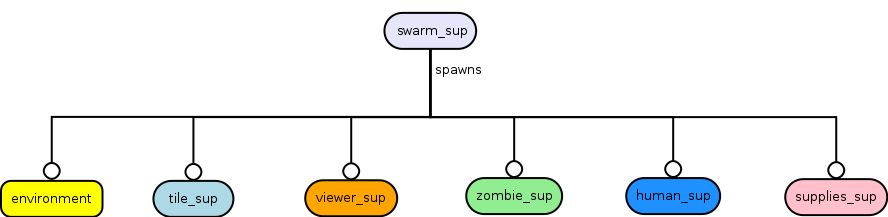
\includegraphics[width=3in]{../img/supervisor.png}
\caption{Supervision Tree for Swarmer}
    \label{fig:sup_tree}
\end{figure}

When launched, the \verb+swarmer+ application creates an instance of the \verb+swarm_server+ module. This is the process reponsible for spawning an instance of \verb+swarm_sup+, the systems main supervisor process, and an instance of \verb+swarm_handler+, a Cowboy WebSocket server \cite{cowboy} controller module that manages communication between the the simulation and the client. \verb+swarm_handler+ and the Cowboy Server are covered in more detail in section \ref{client}.\\
\\
The \verb+swarm_sup+ process will create the applications Supervision Tree, shown in figure \ref{fig:sup_tree}. The supervisor spawns an instance of the \verb+environment+ module and the \verb+tile_sup+, \verb+viewer_sup+, \verb+human_sup+, \verb+zombie_sup+, and \verb+supplies_sup+ supervisor processes.\\
\\
The \verb+environment+ module has two main roles within the application. Firstly its job is to set the simulation environment up, covered in section \ref{environment_creation}, and secondly to deal with the regular report requests from the \verb+swarm_handler+ process.\\
\\
The \verb+tile+ and \verb+viewer+ processes will be spawned by their respective supervisors on request from the \verb+environment+. The \verb+tile+ processes provide a two dimensional space in which the entities can move. The \verb+viewer+ processes provide a method for requesting data regarding an entities surroundings. The way this is set up and an explanation of how entities use these facilities will be covered in section \ref{tile_viewer}.\\
\\
Once the simulation environment has been created, the \verb+environment+ process will then spawn a number of zombies, humans and supplies based on the setup parameters received from the \verb+swarm_handler+ process.\\
\\
After initial setup, the full systems' supervision tree would look something like figure \ref{fig:system_ws}, however there would be considerably more child processes in a typical setup of the application.
\begin{figure}[h]
  \centering
  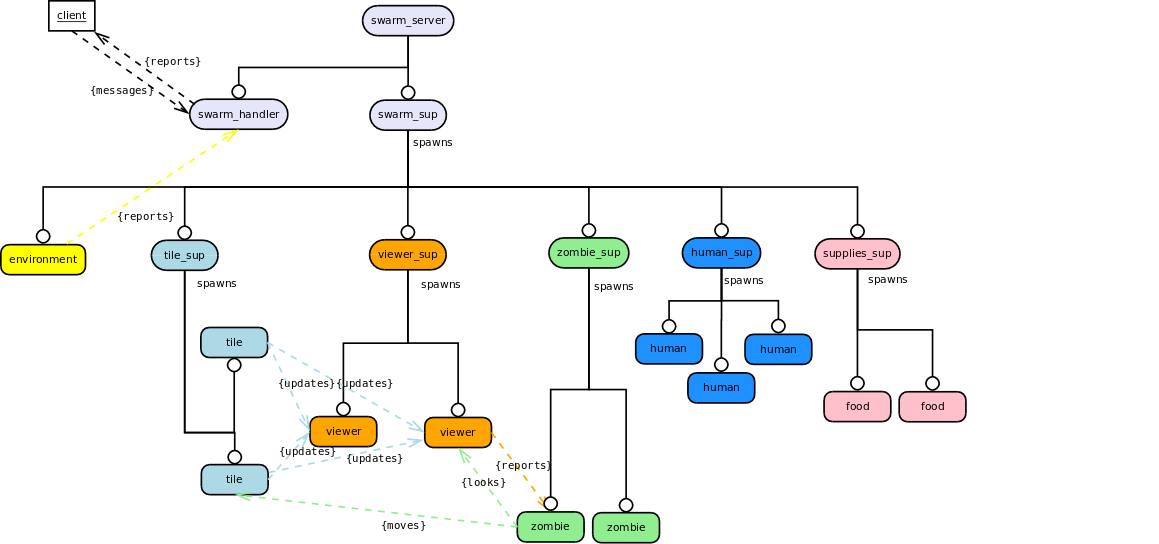
\includegraphics[width=4in]{../img/final_system_ws.png}
\caption{System Architecture}
    \label{fig:system_ws}
\end{figure}

\section{The Tile-Viewer System \label{tile_viewer}}
One of the main features of the concurrent system is the tile-viewer mechanism that we have implemented. Each tile represents two dimensional area of space, and keeps track of the entities acting within it. The tile communicates updates to its own viewer, and each viewer of the tiles neighbourhood. The relationship between a tile and its viewers is depicted in figure \ref{fig:tile_viewer_rel} and the method of assigning viewers to tiles to create a neighbourhood is explained in section \ref{environment_creation}.
\begin{figure}[h]
  \centering
  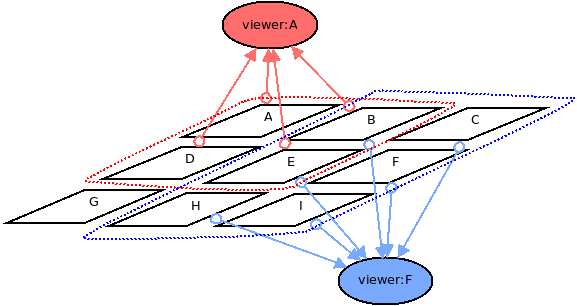
\includegraphics[width=2.5in]{../img/tile_to_viewer_map.png}
  \caption{Tile Viewer Relationship}
  \label{fig:tile_viewer_rel}
\end{figure}

A \verb+viewer+ process provides a means for entities to look into neighbouring tiles. The \verb+viewer+ has functions which return lists containing information about entities and obstructions. The main reason for seperating the \verb+tile+ and \verb+viewer+ processes is to allow for a more efficient concurrent design. One of the problems we came across early on in the project arose because initially we had entities requesting both new positions from the tile and requesting information from it at another time. This lead to, too many messages being passed between the tiles and entities. This resulted in deadlocks. Having a seperate \verb+viewer+ and \verb+tile+ allows for position requests and information requests to be handled independently, limiting the amount of data held in the \verb+tile+ and removing the chance of a deadlock.

\section{Environment creation \label{environment_creation}}
The creation of an environment begins with the setting of a value for the number of tiles in the grid. As all of our grids are square, there is only a single value for the dimensions of the array. The size of the tile array is determined from the size of the obstruction map selected (section: \ref{obstructions}). Once the dimensionality has been obtained, the grid is constructed through a recursive call to \verb+environment:make_row+ to create an full set of tile processes and corresponding viewer processes. Every tile process is assigned a unique dynamically generated name, which can be used to identify the column and row the tile is positioned in. Tiles can then be identified by using a pair of coordinates to derive a tile id. The ability to derive the appropriate tile id through a function call containing coordinates is one of the keys to our systems flexibility and the ease of adding new features.\footnote{Tile names are Erlang atoms registered in the supervision tree of the form tileX0Y0}\\
\\
The next stage involves creating a list for each tile of all its neighbouring viewers. Finally, obstructions and entities are added to each completed tiles state. The system will now be in a paused state, ready to run the simulation.\\

\section{Obstructions \label{obstructions}}
Although we had always planned to include obstructions within our environment, the functionality was a late addition to the simulation. We were concerned with how the resolution would affect our planned inclusion of heuristic path planning.\footnote{Heuristic path planning was one of our unrealised stretch goals.} We decided to implement obstructions at a fraction of the natural simulation resolution. As we had previously fixed the size of environment tiles at \(50^2\) we selected a size of \(5^2\) for each cell of the \emph{obstruction grid}. Obstructed coordinates stored in the tiles state, are on the obstruction grid scale. In a grid 5 tiles by 5 tiles in size, there are \emph{obstruction cells} in the range of \( (0,0) \) to \( (49,49) \).\\
\\
One of our primary considerations was being able draw the environment using a paint tool. We selected mtPaint \footnote{http://mtpaint.sourceforge.net/} due to the ease of exporting images as ascii files.\\
\\
For a standard 5x5 tile environment, we create a plain white image \(50^2\) pixels in size and draw in the required obstructions. See figure \ref{fig:mtpaint}.\\

\begin{figure}[h]
  \centering
  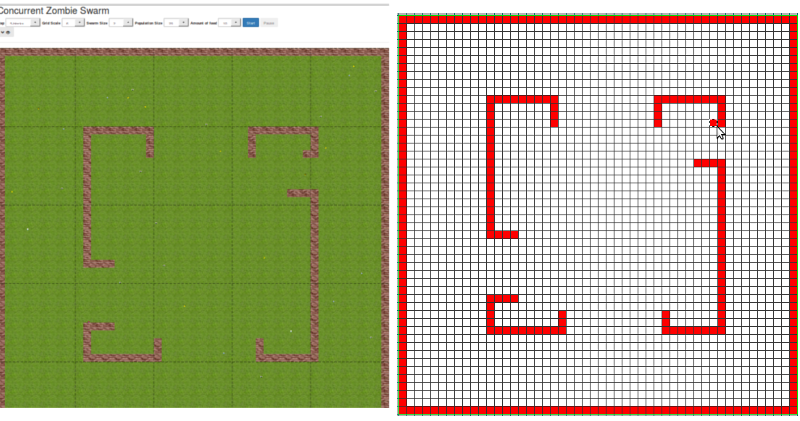
\includegraphics[width=2.5in]{../img/mt_paint.png}
\caption{Mt Paint}
    \label{fig:mtpaint}
\end{figure}

The resulting ascii file, stripped of line breaks, produces a string of 2500 characters. The string is then processed into an array of indices corresponding to the positions of obstructions. In order to convert an index back into a coordinate pair (on the obstruction grid scale) where \(I\) is the index obtained using \(X = I mod 10\) and \(Y = I / 10\).\\
\\
Once the coordinates have been obtained, the corresponding tile id can be identified using \(X / 10\) and \(Y / 10\). Each tile contains the subset of obstructions which corresponds to its own geometry. Whenever an entity wishes to perform an operation over the obstruction grid scale, the coordinates are simply divided by 5 and compared against the tiles record. This system provides a flexible resolution independant method of modelling obstructions. Although we haven't parameterised the scale of the obstruction grid, it would be trivial to add this functionality.

\section{Entity Intelligence \label{behaviours}}
Both the human and zombie entities are modelled using algorithms based on the Boids flocking model. Although both algorithms are heavily modified from the basic definition of a Boids model and from each other they, both share a certain amounts of functionality. For instance, both entities share movement methods, flocking functions, obstacle evasion, and elements of the descision making process.\\

\subsection{PSO \label{pso}}
Before settling on our current Boids-based implementation for zombie intelligence, we implemented behaviours based on Particle Swarm Optimisation\cite{pso} (PSO). PSO is a population based algorithm which optimises a populations mean fitness, in this case towards the shortest distance to target entities.\\
\\
In this implementation the zombies would obtain a list of entities within their viewer and then sort the list according to distance and truncate it to only include those entities within sight. The zombie would then move towards the closest human target if there is one in sight, however if there is not one then they will move towards the highest fitness zombie that they can detect. \footnote{i.e. the zombie closest to a human entity} Using this, the zombie population will optimise towards the position of the nearest human entity.\\
\\
While this implementation did allow for the zombies to chase humans and appear to move as a group, it did not produce much emergent behaviour and the idea of global fitness did not work well with our goal of creating a realistic zombie swarm.\\
\\
After some deliberation we decided it would be best if we took what we had learnt and implemented for PSO and use it to create a more interesting and realistic simulation using flocking algorithms.\\

\subsection{Entity Movement \label{movement}}
Our final Boids-based entities use a coordinate system to determine their positions. Each entity has an integer value of X and Y, representing its represents its location in space. Entities also calculate a velocity for the X axis and Y axis, these velocities can be positive or negative, allowing movement in any direction, these values do not have to be integers which allow velocities to naturally increase or decrease over time.\\
\\
Every time an entity makes a decision, it will result in a change of velocity. The new velocity is then summed with the current coordinates of the entity \footnote{i.e. the X velocity is added to the X coordinate and the Y velocity to the Y coordinate} to determine the entities new proposed location.\\

\subsection{Making Decisions \label{desicions}}
Entities have to make a decision on where to move every time they make an action. To make this decision the entities need to know which other entities are within their sensory range and what distance away they are. To find this out, an entity requires two lists, one for zombies and one for humans. The entities query their viewer to create these lists. The entity then calculate the difference in position between them each entity, then cuts down the lists to remove any entities too far away to be visible and to remove entities that are not visible due to obstructions, finally the entity sorts the lists by distance.\\
\\
The entities then pattern match using the contents of these lists to decide what move to make.\\

\begin{figure}[h]
  \centering
  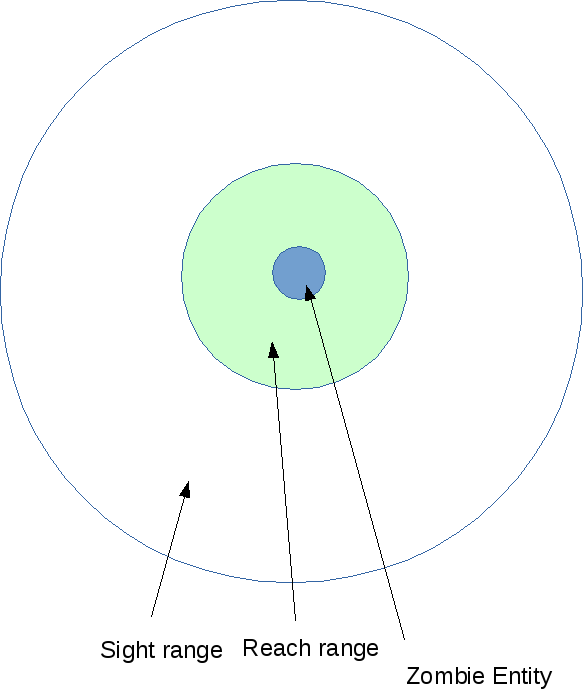
\includegraphics[width=2in]{../img/zombie_range.png}
\caption{A Zombies Line of Sight}
    \label{fig:zombie_los}
\end{figure}

\subsection{Priorities \label{priorities}}
Both humans and zombies make decisions on where to move using a pattern matching function called \verb+make_choice+. This function takes, as arguments, lists of all humans and zombies in sight to match against different cases. Because it is inevitable for multiple cases to be true at the same time, the entities have to prioritise certain matched patterns over others. For example, having a zombie within reach also means that a zombie would be within sight, in this case the reaction for having a zombie within reach would take priority.\\

\begin{figure}[h]
  \centering
  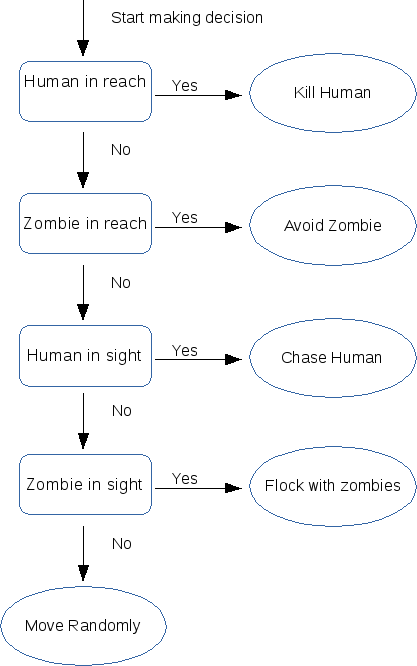
\includegraphics[width=2in]{../img/zombie_decision_tree.png}
\caption{A zombies Desicion Tree}
    \label{fig:zomb_tree}
\end{figure}

Although the method is very similar between the different entities, there are very important differences in the way they prioritise the pattern matching. In a zombie, being able to reach and attack a human takes priority above all other cases. The next highest priority would be avoiding collision with other zombies within reach, then chasing after humans in sight. Finally, flocking with other zombies near it. A zombies priority tree is shown in figure \ref{fig:zomb_tree}.\\
\\
In a human, avoiding collision with other entities takes priority in order to represent a humans spacial awareness. Following this, a human would attempt to run away from zombies, and look for food before attempting to flock with other humans.\\
\\
The outcome of this is that the humans and zombies are able to exhibit considerably different behaviours, with only a few changes to the order of priorities.\\

\section{Obstacles \label{obstacles_b}}
A major factor in creating more interesting behaviours in our entities is the possibility of areas of the maps being obstructed. There are two kinds of obstacles that can affect the behaviour of an entity, other entities and built-in obstructions in the map. Once an entity has chosen a new set of coordinates. These coordinates are then checked, by the tile they wish to move onto, to ensure they unobstructed and constiture a legal move. This is shown in figure \ref{fig:obs_los}.\\
\begin{figure}[h]
  \centering
  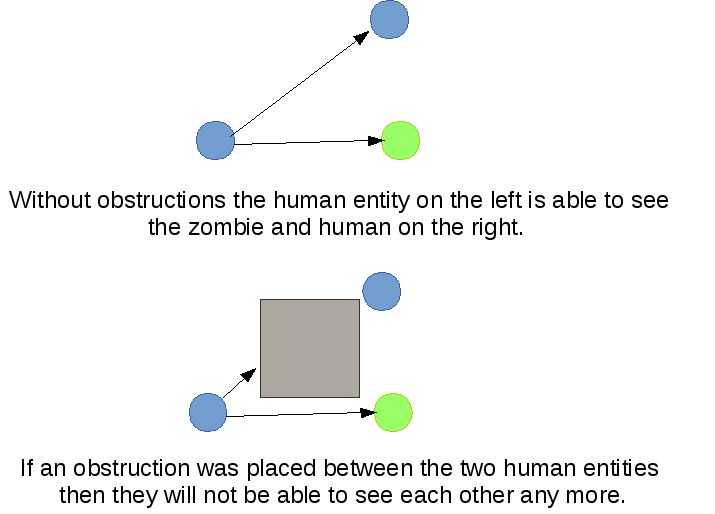
\includegraphics[width=2in]{../img/los_demo.png}
\caption{Line of Sight}
    \label{fig:obs_los}
\end{figure}
\\
Due to the concurrent nature of our simulation, it is possible for two entities to want to occupy the same coordinate. If this happens then the second entity will bounce off of the first entity. The bouncing entity, calculates its new position using its current velocities to work out the angle of collision and then moving to a coordinate 1 space away from its target, at either the opposite angle or 45 degrees from that. eg. If an entity collides with another from below, it will end up one space below the target, one space below and right or one space below and left.\\
\\
Obstructions work a little differently from entity obstacles, The entity will again calculate the angle of collison, but instead of bouncing off the obstruction, the entity will reset its velocity along the axis in which it hit the obstruction causing it to start moving in the opposite direction while staying on its original course in the other axis. This allows the entities to maintain velocity in one axis, while obstructed in another.\\
\\
Obstructions also have another effect on the entities, they can block line of sight. What this means is, although entities may be within range to see each other, if there is an obstruction somewhere along the direct line between them, neither entity can be aware of the others presence. In effect obstructions act as walls that block both the movement and the sight of entities.\\

\section{Food and Energy \label{food}}
There is one other main difference between zombie and human entities. Both types of entities have an energy value which gradually decreases over time. When the energy of a human or zombie falls below a certain threshold, the entity will have a lower limit placed on its speed, causing it to slow down due to hunger. To recover energy both zombies and humans have to eat.\\
\\
For a zombie, eating happens by killing and converting a human entity into a zombie, zombies have no changes in behaviour caused by hunger as they always want to kill humans and lack the intelligence to consider saving meals until they are hungry.\\
\\
Humans on the other hand have a much more interesting relationship with food, there are several food items placed on the map at the beginning of the simulation which humans can pick up to recover energy. However humans do not seek this food out until they have become very hungry. Once they have become very hungry the human behaviour changes to actively seek out food, while they will continue to avoid zombies and other humans that are close to, they will also start trying collect food that they have previously discovered the location of, to restore thier energy.\\

\section{Zombifying Humans \label{zombifying}}
When a zombie manages to get close enough to a human then the zombie will attempt to attack the human. There is a chance that the zombie will succeed in his attack, if this happens then the zombie passes a message to the human causing it to terminate and spawning a new zombie process in humans previous position.\\

\section{Client Visualisation \label{client}}
\label{visualisation}
The use of a decoupled client to visualise the state of the simulation was one of the very early goals specified in the project. One of the main reasons we decided to do things this way is the lack of graphical API's native to Erlang. The use of a solution based on HTML and JavaScript has allowed the development of client which connects to the simulation over a network, easing the computational burden on the machine running the simulation.\\
\\
The first stage in establishing a client/server model was passing environmental data over the network. We chose to use a WebSocket based approach early on due to it duplex functionality, although with hindsight, plain HTTP requests would have more than likely sufficed.\\
\\
The development of the client required the learning of new JavaScript libraries (Angular.js and D3.js) and research into WebSockets. On the Erlang side we utilised the Cowboy WebSocket\cite{cowboy} server and JSX, JSON encoder libraries. JSON objects are decoded and the \verb+type+ attribute is matched against a case statement in the WebSocket handler. In this way various types of control messages can be recognised and appropriate actions propagated throughout the environment. When the client HTML page loads, a setup - typed, JSON message is fired off to create a default environment, populated with randomly placed entities. Each time a user alters a parameter a new JSON setup object is submitted and the returned environmental data visualised. New environments are created with all entities paused.\\
\\
By ensuring only data returned over the WebSocket connection is visualised, we ensure that what we see in the visualisation is actually being represented in the simulation. The use the D3.js library as the basis for mapping simulation data to visual elements enforced the use of a Scalable Vector Graphic (SVG) as the main component of visualisation. This worked out very well as SVG images are entirely specified in XML, allowing the mapping of arbitrary attributes to elements. For example Zombies visualised in the SVG are \verb+<image>+ elements but have attributes such as \verb+x_vel+, unused in the visualisation but very helpful in debugging and testing the system. Other niceties of the SVG format include facilities such as mapping Erlang process ids to element \verb+id+ attributes as in fig \ref{fig:svg_elements}

\begin{figure}[h]
  \centering
  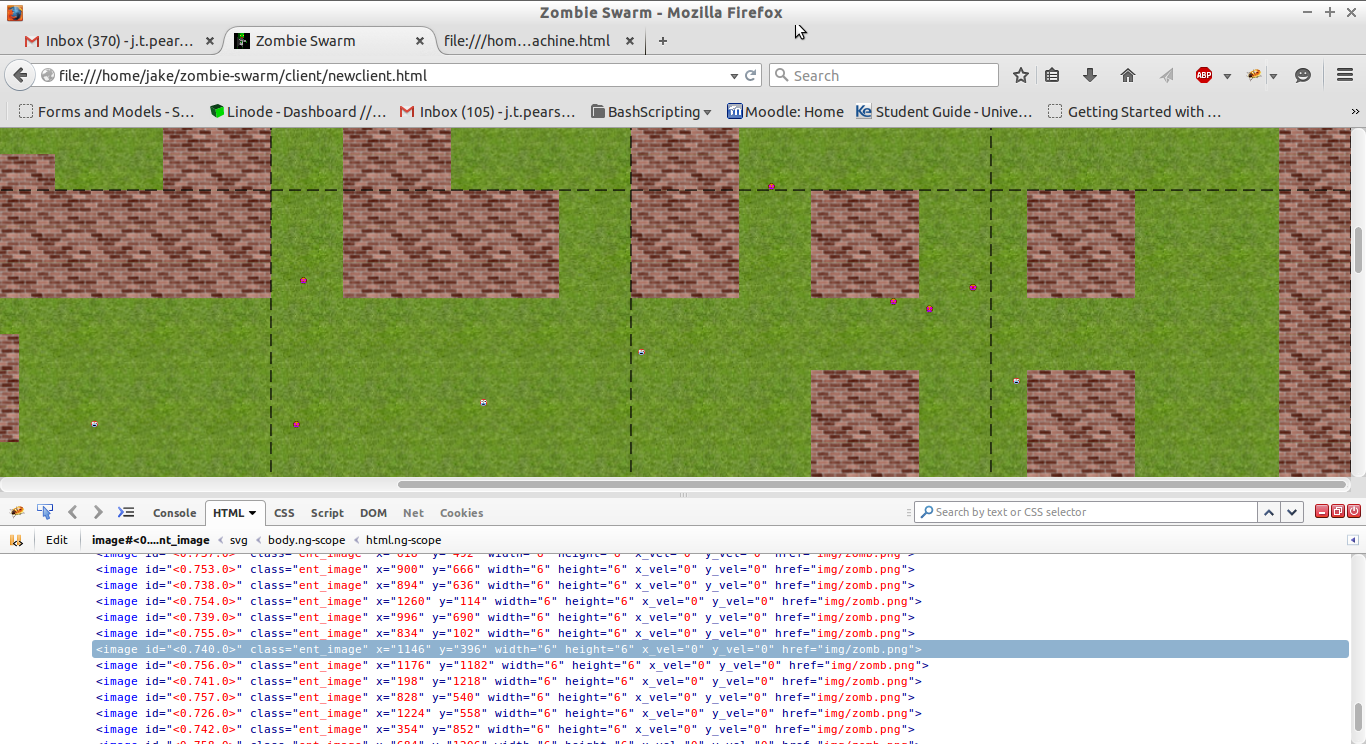
\includegraphics[width=3in]{../img/element_attributes.png}
  \caption{Arbitrary attributes mapped to SVG elements}
    \label{fig:svg_elements}
\end{figure}

The main event loop is entered by clicking on a "start" button in the client, causing an unpause message to be propagated through the simulation, one unusal effect arising from the pausing and unpausing of the system in this way (by pausing individual entities) is a slight delay in the propagation of pause/unpause messages resulting in a staggered pause rather than a 'hard' pause. While the main loop is running the client repeatedly sends a \verb+report+ type message over the WebSocket and updates the SVG with the returned data. There are some interesting effects of attempting to visualise a highly concurrent system in necessarily discrete steps such as discrepancies between entity states and tile states. These type of discrepancies are inherent in the design of the system and naturally resolve themselves but they are captured at the instant of visualisation.

\section{Conclusion}

% what we have not managed to implement

The aim of the project was to create a highly concurrent simulation of swarm intelligence, in which zombie and human entities interact within an environment. We wanted the simulation to exhibit complex, emergent behaviours arising from simple sets of instructions.\\
\\
Overall, the project has been a success. By observing the simulation running you can see a number of interesting situational behaviours. Behaviours that we have observed are:
\begin{itemize}
    \item Swarms interact with obstructions in interesting ways. When the swarm collides with an obstruction, it can disperse around the edges of the obstacle. Sometimes the swarm will regroup on the other side, however this may not happen due to the shape of the obstacle or other stimulus taking priority.
    \item Due to the effect of inertia simulated through velocity, entities can be observed acclererating, decelarating and changing direction by swerving. \item Energy levels have a noticable effect on the simulation over its lifetime. Early on in the simulation, humans have a higher survival rate because they can move faster. However, as food becomes scarce, humans will slow down over time. Humans caught early on in the simulation tend to have been cornered by a zombie, or surrounded.
    \item It is possible for a group of humans to find a 'safe-zone' in the simulation. This can allow humans to hide from the zombies behind obstacles  for an extended period of time, however they will eat all of the food in the area, and when a zombie swarm does discover them, it is likely that they will be too slow to escape.
    \item When humans pass within range of a zombies on the edge of a swarm, somtimes only the zombies on the edge of the swarm move towards the humans initially. This can lead to just a few zombies breaking away from the main swarm, or lead to a chain reaction in which the entire swarm will follow. This depends on what stimulus other members of the swarm are able to detect.
    \item When there is a large population of humans, and not many obstacles to break the line of sight across the environment, this can lead to the zombies forming a line sweeping across the environment.
\end{itemize}

Unfortunately there were certain elements of the system that we were not able to create, due a combination of time preassure and the level of difficulty. The main one was a full heuristic pathfinding algorithm for humans. Though this is partially implemented as part of the submission, we did not have time fully explore and test this element of the application, we do not know to what extent it is functioning.

\section{Acknowledgements}
We would like to thank Dr. Peter Kenney for supervising this project, and providing valuable input on designing and implementing the two dimentional space simulation, as well as helping us design and understand our Boids algorithm.\\
\\
We would also like to thank Dr. Fred Barnes on the invaluable help with desiging our concurrent architecture.

% references section

% can use a bibliography generated by BibTeX as a .bbl file
% BibTeX documentation can be easily obtained at:
% http://www.ctan.org/tex-archive/biblio/bibtex/contrib/doc/
% The IEEEtran BibTeX style support page is at:
% http://www.michaelshell.org/tex/ieeetran/bibtex/
%\bibliographystyle{IEEEtran}
% argument is your BibTeX string definitions and bibliography database(s)
%\bibliography{IEEEabrv,../bib/paper}
%
% <OR> manually copy in the resultant .bbl file
% set second argument of \begin to the number of references
% (used to reserve space for the reference number labels box)
\begin{thebibliography}{1}

  \bibitem{erlang}
    Ericsson AB,
    \emph{About Erlang},
    \url{http://www.erlang.org/about.html}

  \bibitem{d3}
    Mike Bostock,
    \emph{D3 Website},
    \url{http://d3js.org/}

  \bibitem{occam_boids}
    Fred Barns,
    \emph{GPU Boids},
    \url{http://frmb.org/occam.html#gpuboids}

  \bibitem{erlang_boids}
    Jim Menard,
    \emph{Erlang Boids Simulation Design},
    \url{http://jimmenard.blogspot.co.uk/2007/06/erlang-boids-simulation-design.html}

  \bibitem{boids}
    Craig Reynolds,
    \emph{Boids - Background and Update},
    \url{http://www.red3d.com/cwr/boids/}

  \bibitem{otp}
    Ericsson AB,
	  \emph{Open Telecom Platform Design Principles},
    \url{http://www.erlang.org/doc/design_principles/sup_princ.html}

  \bibitem{supervisors}
    Ericsson AB,
	  \emph{Erlang Supervisors},
    \url{http://www.erlang.org/doc/man/supervisor.html}

  \bibitem{gen_server}
    Ericsson AB,
	  \emph{Erlang Generic Servers},
    \url{http://www.erlang.org/doc/Design_principles/gen_server_concepts.html}

  \bibitem{gen_fsm}
    Ericsson AB,
	  \emph{Erlang Generic Finite State Machines},
    \url{http://www.erlang.org/doc/design_principles/fsm.html}

  \bibitem{cowboy}
    Nine Nines,
    \emph{An Introduction to Cowboy},
    \url{http://ninenines.eu/docs/en/cowboy/1.0/guide/introduction/}

  \bibitem{pso}
    Kennedy, J.; Eberhart, R. (1995),
    \emph{Particle Swarm Optimization},
    Proceedings of IEEE International Conference on Neural Networks IV,
    pp. 1942–1948

\end{thebibliography}

% that's all folks
\end{document}
